%! TEX root = ../main.tex
In this section, we measure wealth inequality in Chile. In particular, we analyze the 2021 cross-section using data from the Household Financial Survey (\textit{Encuesta Financiera de Hogares}, EFH) published by the Central Bank of Chile \citep{bcentral2021efh}.

To account for differential unit non-response and extreme under-reporting at the upper tail of the wealth distribution, a pervasive limitation of survey data, we implement the tail-correction methodology developed by \citet{vermeulen2018}. Specifically, this approach fits a Pareto distribution to the tail by combining survey observations with external data on ultra-high-net-worth individuals from the \textit{Forbes World's Billionaires} list \citep{forbes2021billionaires,forbes2021kaggle}.

Finally, we compare the baseline survey estimates with the Pareto-corrected wealth shares and discuss the sensitivity of the results.

\subsection{Measuring wealth inequality}\label{sec:measuring-wealth}
Following standard international guidelines \citep[e.g.,][]{oecd2013wealth} and the methodology of the Central Bank of Chile for the EFH, net wealth (or net worth) of household $i$, denoted by $W_i$, is defined as the total value of all its non-financial and financial assets minus total outstanding liabilities:
\begin{equation}
    W_i = A_i - L_i = (A_i^{\text{NF}} + A_i^{\text{F}}) - (L_i^{\text{M}} + L_i^{\text{NM}}),
    \label{eq:net_wealth}
\end{equation}
where:
\begin{itemize}
    \item $A_i^{\text{NF}}$ denotes \textit{non-financial assets}, primarily comprising main residence, secondary real estate properties, and other tangible assets (vehicles, machinery, and self-employment business assets).
    \item $A_i^{\text{F}}$ denotes \textit{financial assets}, including checking and savings accounts, mutual and pension funds (voluntary retirement savings), stocks, bonds, and business equity holdings.
    \item $L_i^{\text{M}}$ represents \textit{mortgage debt} secured against real estate (housing and other properties).
    \item $L_i^{\text{NM}}$ represents \textit{non-mortgage liabilities}, covering consumer loans, credit cards, education debt, and informal or retail commercial credit.
\end{itemize}
Under this definition, gross wealth is $A_i = A_i^{\text{NF}} + A_i^{\text{F}}$, and net wealth $W_i$ can be negative for over-indebted households ($L_i > A_i$). 

Three main empirical and methodological challenges arise when measuring wealth inequality under this framework. First, wealth is substantially more concentrated than income because it accumulates over the life cycle and across generations. Consequently, the wealth distribution exhibits a fat Pareto tail, meaning that undersampling or non-response among the wealthiest households exerts a first-order downward bias on inequality estimates. Second, measuring wealth components through surveys is subject to severe measurement error and item non-response, requiring complex imputation procedures that inevitably introduce estimation uncertainty. Third, because net wealth can take negative values, standard summary indices such as the Gini coefficient \citep{gini1912variabilita} lose some of their desirable axiomatic properties (e.g., boundedness between 0 and 1; see Appendix \ref{app:gini-negative} for a mathematical proof). To face this, the empirical literature primarily relies on percentile wealth shares (such as the share of wealth held by the top 1\% or 10\%), 
\begin{equation}
    S_P = \frac{\sum_{i=1}^N w_i W_i \cdot \mathbf{1}\{W_i \in P\}}{\sum_{i=1}^N w_i W_i},
    \label{eq:wealth_share}
\end{equation}
where $w_i$ denotes the survey sampling weight of household $i$, $\mathbf{1}\{\cdot\}$ is the indicator function, and $P$ represents the subset of households belonging to a specific percentile bracket (e.g., the top 1\%, top 10\%, or bottom 50\%).

While wealth shares directly capture concentration at key points of the distribution, they do not provide a single scalar summary of dispersion across the entire population. In this context, reporting the wealth share of the bottom 50\% is essential to provide a balanced assessment of concentration and to evaluate disparity across the entire distribution. 

Because positive and negative net wealth values offset each other in the summation, the survey-based aggregate denominator ($\sum_{i=1}^N w_i W_i$) can become highly volatile or sensitive to extreme debts. Household surveys also systematically under-report aggregate financial and non-financial assets relative to macroeconomic totals. To address these limitations and follow standard distribution national accounts (DINA) practices, we anchor the denominator to the aggregate household net wealth reported in the National Accounts by the Central Bank of Chile \citep{bcentral2021financialaccounts}. The rescaled wealth share is thus defined as:
\begin{equation}
    S_P^{\text{NA}} = \frac{\sum_{i=1}^N w_i W_i \cdot \mathbf{1}\{W_i \in P\}}{W^{\text{NA}}},
    \label{eq:wealth_share_na}
\end{equation}
where $W^{\text{NA}}$ denotes the total household net wealth benchmark from the National Accounts. 

\subsection{Addressing the Differential Unit Non-Response Problem}\label{sec:vermeulen}
Sample surveys suffer from missing data at the upper tail because ultra-wealthy individuals exhibit disproportionately higher unit non-response rates and under-report sensitive assets (Section~\ref{sec:measuring-wealth}). To correct for this truncation and obtain an accurate representation of top wealth shares, \citet{vermeulen2018} proposed a semi-parametric tail-correction methodology that augments survey microdata with external rich lists (such as the \textit{Forbes World's Billionaires} rankings) and estimates an augmented Pareto distribution.

Because power-law behavior holds strictly at the upper tail, the Pareto model is fitted only for wealth levels exceeding a predetermined lower threshold, $w_{\min}$ (see Appendix \ref{app:pareto-foundations} for microeconomic foundations). In practice, $w_{\min}$ is chosen based on visual inspection of log-log rank plots (detecting where the linearity of the tail begins) or through goodness-of-fit heuristics \citep[e.g.,][]{clauset2009power,vermeulen2018}.

Formally, for any wealth level $w \ge w_{\min}$, the cumulative distribution function (CDF), denoted by $F(w)$, and the probability density function (PDF), denoted by $f(w)$, of a Type-I Pareto distribution are defined as:
\begin{align}
    F(w) &= 1 - \left(\frac{w_{\min}}{w}\right)^\alpha, \label{eq:pareto_cdf} \\
    f(w) &= \frac{\mathrm{d}F(w)}{\mathrm{d}w} = \frac{\alpha w_{\min}^\alpha}{w^{\alpha + 1}}, \label{eq:pareto_pdf}
\end{align}
where $w_{\min} > 0$ represents the tail cutoff point and $\alpha > 0$ is the Pareto shape parameter (tail index), governing the thickness of the tail (with smaller values of $\alpha$ indicating a heavier tail and higher wealth concentration). The complementary cumulative distribution function (or survival function), which gives the probability that an individual's wealth exceeds $w$, is therefore expressed as:
\begin{equation}
    P(W > w) = 1 - F(w) = \left(\frac{w_{\min}}{w}\right)^\alpha.
    \label{eq:pareto_survival}
\end{equation}

The estimation and imputation procedure is summarized in Algorithm \ref{alg:vermeulen}. To estimate the Pareto tail index $\alpha$, we apply the pseudo-maximum likelihood (PML) estimator developed by \citet{vermeulen2018}. Standard Maximum Likelihood cannot be applied directly because survey observations represent sampled clusters with expansion weights $w_i$, whereas the Forbes list represents an exhaustive, unweighted census ($w_j^F = 1$) of extreme wealth. The PML log-likelihood function combines both data sources by weighting each survey contribution by its sampling weight while treating billionaire records as self-representing:
\begin{equation}
    \ln \mathcal{L}(\alpha) = \sum_{k=1}^n w_k \ln f(W_k; \alpha) + \sum_{j=1}^M \ln f(W_j^F; \alpha).
    \label{eq:pml_loglik}
\end{equation}
Substituting the Pareto density $f(w; \alpha) = \alpha w_{\min}^\alpha w^{-(\alpha + 1)}$ and solving the first-order condition $\frac{\partial \ln \mathcal{L}}{\partial \alpha} = 0$ yields the closed-form estimator:
\begin{equation}
    \hat{\alpha} = \frac{\sum_{k=1}^n w_k + M}{\sum_{k=1}^n w_k \ln\left(\frac{W_k}{w_{\min}}\right) + \sum_{j=1}^M \ln\left(\frac{W_j^F}{w_{\min}}\right)}.
    \label{eq:alpha_pml}
\end{equation}
Econometrically, $\hat{\alpha}^{-1}$ corresponds to the weighted average relative distance of log wealth above the cutoff $w_{\min}$. When wealth in the tail is heavily concentrated far above $w_{\min}$, the denominator expands, resulting in a lower $\hat{\alpha}$ (i.e., a heavier Pareto tail, which implies a higher concentration of aggregate wealth and greater inequality).

As a complement to PML, we also use the bias-corrected rank-size regression of \citet{gabaix2011rank}\footnote{See \texttt{source/pareto.py:L5-L38} (\texttt{estimate\_alpha\_pareto}, \texttt{method="reg"}).}. Sorting the combined tail sample descending with cumulative weights $R_k$, the Pareto implies $\ln(R_k/N)\approx -\alpha\ln(W_k)+\alpha\ln w_{\min}$, so $\alpha$ is minus the OLS slope of log-rank on log-wealth. We use the $1/2$ shift, $\ln((R_k-0.5w_k)/N)$ on $\ln W_k$, to reduce small-sample bias at the very top.

\begin{algorithm}[H]
    \caption{Vermeulen (2018) Tail-Correction Procedure}\label{alg:vermeulen}
    \SetAlgoLined
    \KwIn{Survey microdata $\{(W_i, w_i)\}_{i=1}^N$; external Forbes list $\{W_j^F\}_{j=1}^M$; tail threshold $w_{\min}$; national accounts benchmark $W^{\text{NA}}$.}
    \KwOut{Pareto tail index $\hat{\alpha}$; pseudo-observations with weights; corrected top wealth shares $\hat{S}_P$.}
    
    \BlankLine
    \tcp{Step 1: Sample Selection above Tail Threshold}
    Extract survey households satisfying $W_i \ge w_{\min}$, indexing them by $k = 1, \dots, n$, with weights $w_k$\;
    Include external Forbes individuals with weight $w_j^F = 1$, since they represent the full enumeration of known billionaires ($W_j^F \ge w_{\min}$)\;
    
    \BlankLine
    \tcp{Step 2: Estimation of the Pareto Tail Index ($\alpha$)}
    Fit a Type-I Pareto distribution $P(W \ge w) = (w_{\min} / w)^\alpha$ on the combined sample by pseudo-maximum likelihood (or weighted OLS on the rank log-log regression):
    \[
        \hat{\alpha} = \frac{\sum_{k=1}^n w_k + M}{\sum_{k=1}^n w_k \ln(W_k / w_{\min}) + \sum_{j=1}^M \ln(W_j^F / w_{\min})}
    \]
    
    \BlankLine
    \tcp{Step 3: Replacing or Augmenting the Survey Tail}
    Replace the empirical survey observations above $w_{\min}$ with synthetic pseudo-observations generated from the estimated Pareto density $f(w; \hat{\alpha}) = \hat{\alpha} w_{\min}^{\hat{\alpha}} w^{-(\hat{\alpha}+1)}$, calibrating total population weights to match the aggregate tail mass $N_{\text{tail}} = \sum_{k=1}^n w_k$\;
    
    \BlankLine
    \tcp{Step 4: Recomputing Corrected Wealth Shares}
    Evaluate aggregate tail wealth $\hat{W}_{\text{tail}} = N_{\text{tail}} \cdot \frac{\hat{\alpha}}{\hat{\alpha} - 1} w_{\min}$ (for $\hat{\alpha} > 1$)\;
    Compute the corrected wealth shares using the benchmark denominator $W^{\text{NA}}$ (or total corrected wealth $\hat{W}^{\text{total}} = \sum_{W_i < w_{\min}} w_i W_i + \hat{W}_{\text{tail}}$):
    \[
        \hat{S}_P = \frac{\hat{W}_P}{W^{\text{NA}}}
    \]
\end{algorithm}

% ================================================================================
% ================================================================================
\newpage
\subsection{Results}\label{sec:results}
In this section, we present the empirical results obtained from the implementation of the methodologies described in Sections \ref{sec:measuring-wealth} and \ref{sec:vermeulen}. All scripts and replication materials are available in the GitHub repository \url{https://github.com/crisdonoli/measuring-inequality}. To facilitate replication, key computational steps are referenced in footnotes where appropriate.

\paragraph{Data Preparation and Net Wealth Construction.} 
We utilize the 2021 cross-section of the Household Financial Survey (\textit{Base imputada EFH 2021}), containing an initial sample of $136{,}400$ observations. We first clean the data by dropping records with missing values in total assets (\texttt{act\_toth}, $1{,}051$ missing) and total debt (\texttt{d\_toth}, $546$ missing). These excluded observations represent approximately $1.04\%$ of the sample, leaving a final clean dataset of $N = 134{,}984$ households.\footnote{See \texttt{notebooks/01\_efh\_cleaning.ipynb} and \texttt{notebooks/02\_forbes.ipynb} for the complete data loading and pipeline steps.}

Following the Central Bank of Chile's official definitions, household net wealth ($W_i$) is constructed by aggregating all asset components and subtracting total liabilities:
\begin{equation}
    W_i = A_i^{\text{F}} + A_i^{\text{P}} + A_i^{\text{NF}} - L_i,
    \label{eq:net_wealth_efh}
\end{equation}
where $A_i^{\text{NF}}$ is non-financial assets, $A_i^{\text{F}}$ is financial assets, $A_i^{\text{P}}$ is voluntary pension savings, and $L_i$ is total outstanding liabilities.

Table \ref{tab:efh_summary} reports the unweighted summary statistics of the constructed net wealth variable ($W_i$). The distribution shows substantial dispersion: median net wealth is $52.0$ million CLP, whereas the mean reaches $113.6$ million CLP, indicating pronounced right-skewness. Notably, the minimum value is $-298.1$ million CLP (reflecting over-indebted households) and the maximum reaches $4{,}931.6$ million CLP ($\sim 4.93$ billion CLP).

\begin{table}[H]
    \centering
    \caption{Summary Statistics of Household Net Wealth (EFH 2021)}\label{tab:efh_summary}
    \begin{tabular}{lrr}
        \toprule
        \textbf{Statistic} & \textbf{Value (CLP)} & \textbf{Value (Million CLP)} \\
        \midrule
        Count              & $134{,}984$          & -- \\
        Mean               & $113{,}564{,}500$    & $113.56$ \\
        Standard Deviation & $216{,}993{,}600$    & $216.99$ \\
        Minimum            & $-298{,}130{,}700$   & $-298.13$ \\
        25th Percentile (p25) & $11{,}240{,}170$  & $11.24$ \\
        Median (p50)       & $52{,}000{,}000$     & $52.00$ \\
        75th Percentile (p75) & $122{,}049{,}800$ & $122.05$ \\
        Maximum            & $4{,}931{,}589{,}000$& $4{,}931.59$ \\
        \bottomrule
    \end{tabular}
    \vspace{0.2em}
    \flushleft\footnotesize{\textit{Source:} Author's elaboration based on EFH 2021 (\textit{Base imputada}). All figures in Chilean Pesos (CLP).}
\end{table}

The resulting survey-weighted net wealth distribution among Chilean households is displayed in Figure \ref{fig:chilean-pop}.
\begin{figure}[H]
    \centering
    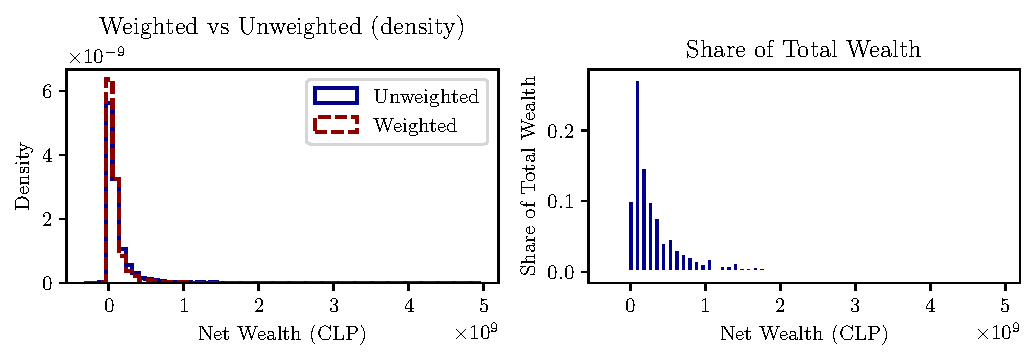
\includegraphics[width=0.95\textwidth]{../../figures/netwealth-efh.pdf}
    \caption{Household Wealth Distribution in Chile (EFH 2021, Survey Weighted)}\label{fig:chilean-pop}
\end{figure}


\paragraph{Measuring Inequality.} Using the distribution above, we calculate percentile wealth shares as defined in Equation \ref{eq:wealth_share}, with households ranked by $W_i$ and weighted by expansion factors $w_i$\footnote{See \texttt{source/shares.py:L5-L35} (\texttt{weighted\_shares}).}. Figure \ref{fig:shares-ineq} reports the baseline survey estimates for the top 1\%, top 10\% and bottom 50\%.
\begin{figure}[H]
    \centering
    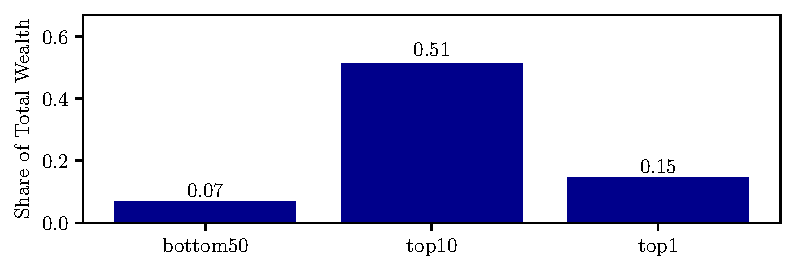
\includegraphics[width=0.85\textwidth]{../../figures/p2/share.pdf}
    \caption{Baseline Wealth Shares in Chile (EFH 2021, No Tail Correction)}\label{fig:shares-ineq}
\end{figure}
These preliminary results show that the top 10\% holds 51\% of total Chilean wealth. However, these shares likely underestimate the top 1\% share because of the differential unit non-response documented in Section~\ref{sec:measuring-wealth}. To address this limitation in the following paragraph we show the results of \citet{vermeulen2018} \footnote{See the whole pipeline in \texttt{notebooks/03\_wealth\_inequality.ipynb} and \texttt{notebooks/04\_vermeulen.ipynb}}.

\paragraph{Forbes Billionaires.} Data on 2021 Chilean billionaires from Forbes is displayed in Figure \ref{fig:billionaires}. We convert USD billions to Chilean pesos using an exchange rate of 759.1 CLP per USD\footnote{See \texttt{source/cleaning.py:L17-L30} (\texttt{convert\_currency}).}.
\begin{figure}[H]
    \centering
    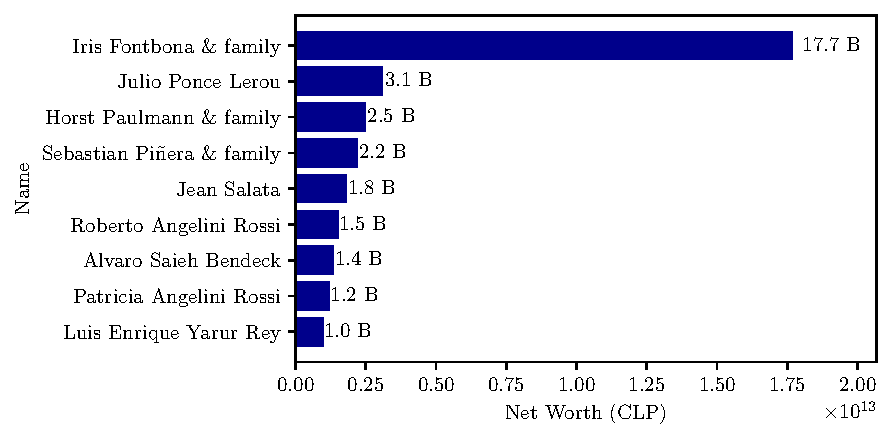
\includegraphics[width=0.90\textwidth]{../../figures/billionaires.pdf}
    \caption{Chilean Billionaires in 2021 (Forbes, Values in CLP)}\label{fig:billionaires}
\end{figure}
Figure \ref{fig:billionaires} is highly skewed: Iris Fontbona holds CLP~17.7~trillion, almost six times the wealth of the remaining eight billionaires in the 2021 Forbes list for Chile.

\paragraph{National Accounts.} Following Equation \ref{eq:wealth_share_na}, we anchor survey aggregates to the December-2021 financial balance for households and non-profit institutions serving households (NPISH)\footnote{File \texttt{data/BDE/CCNN\_CFT\_S14\_AF\_2018.xlsx}, sheet \texttt{Cuadro}, row \texttt{I. Activos Financieros}, December-2021 column; see also \citep{bcentral2021financialaccounts}.}. Let $A^{\text{F,EFH}}=\sum_i w_i A^{\text{F}}_i$ be the survey-weighted financial-asset total and $A^{\text{F,NA}}=426{,}112.5$ billion CLP the macro total; the uprating factor is $\lambda^{\text{F}}=A^{\text{F,NA}}/A^{\text{F,EFH}}$\footnote{See \texttt{source/pareto.py:L83-L107} (\texttt{uprate}).}. We rescale $A^{\text{F}}_i$ by $\lambda^{\text{F}}$ and rebuild $W_i$, so the corrected shares use $W^{\text{NA}}$ as denominator. In 2021 $\lambda^{\text{F}}\approx 0.48$, i.e.\ the survey overstates financial assets relative to the balance-sheet benchmark once pensions are treated separately.

\paragraph{Setting $w_{\min}$ the starting point of the tail.} The cutoff $w_{\min}$ is the wealth level above which power-law behavior is assumed. We set it endogenously as the 99th percentile of the survey-weighted wealth distribution\footnote{See \texttt{source/pareto.py:L131-L147} (\texttt{\_wmin\_from\_percentile}).}, following the survey practice of fitting the tail only at the very top. 

In 2021, $w_{\min}$ ranges from CLP 380--760 million depending on specification, i.e.\ whether we fix it exogenously at USD 0.5m ($\approx$ CLP 380m at 759.1 CLP/USD) or USD 1m ($\approx$ CLP 759m), or set it endogenously as the survey-weighted p99, so we report sensitivity across these three cutoffs. Figure \ref{fig:alpha-sensitivity} shows the estimated tail index falls as the cutoff is lowered: the MLE rises from 1.86 at CLP 380m to 2.53 at the p99, while the regression estimator is stable around 2.13--2.16.
\begin{figure}[H]
    \centering
    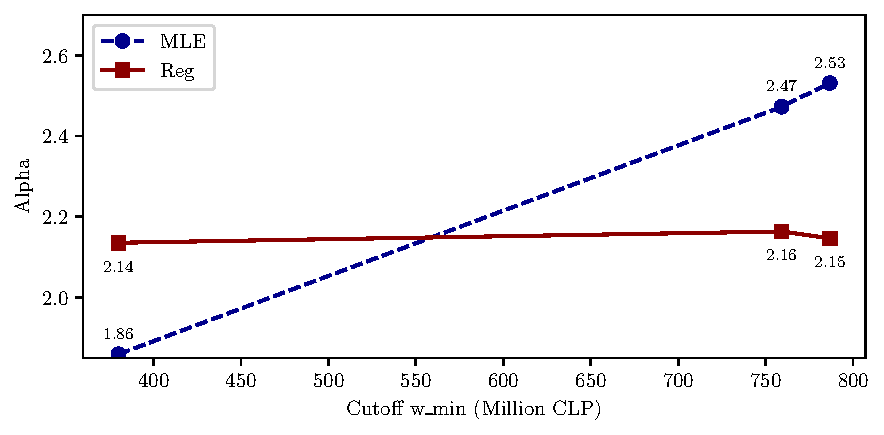
\includegraphics[width=0.85\textwidth]{../../figures/p2/alpha_sensitivity.pdf}
    \caption{Sensitivity of $\hat{\alpha}$ to $w_{\min}$ (MLE vs.\ Regression)}\label{fig:alpha-sensitivity}
\end{figure}

The choice matters because $\hat{\alpha}$ and the corrected top shares move with $w_{\min}$. There is no consensus on an optimal data-driven rule: in practice $w_{\min}$ is chosen by visual inspection of log-log rank plots or goodness-of-fit heuristics \citep[e.g.,][]{clauset2009power,vermeulen2018}, and finding an optimal selector remains an open problem in the literature.

\paragraph{Vermeulen correction.} We fill the gap $[\max(\text{EFH})\approx 4.9\text{b}, \min(\text{Forbes})\approx 987\text{b}]$ with Pareto draws $w = w_{\min}(1-U)^{-1/\hat{\alpha}}$ plus the 9 Forbes records\footnote{See \texttt{source/pareto.py:L148-L187} (\texttt{vermeulen\_correction}).}. As shown in Figure~\ref{fig:pareto_qq}, the MLE slope with $\hat{\alpha}_{\min}\approx 1.85$ (380m cutoff) tracks the empirical points closely, while steeper MLE slopes ($\hat{\alpha}_{\max}\approx 2.53$ at p99) fall below them. By contrast, the Reg panel in the same Figure~\ref{fig:pareto_qq} shows a narrow band ($\approx 2.13$--$2.16$) because $\hat{\alpha}_{\text{Reg}}$ barely moves with $w_{\min}$, so both lines nearly overlap. Figure~\ref{fig:ver_tail} translates this into mass: EFH raw (dashed) truncates at 4.9b, while Vermeulen (solid) bridges the empty gap and extends to 17.7t.

\begin{figure}[H]
    \centering
    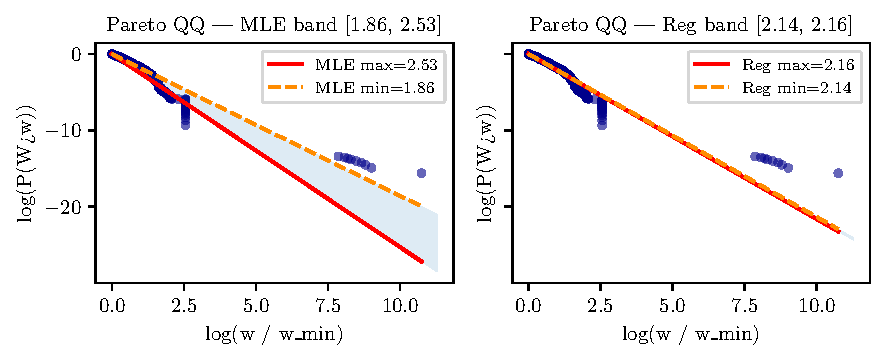
\includegraphics[width=0.95\textwidth]{../../figures/p2/pareto_qq.pdf}
    \caption{Pareto QQ at $w_{\min}=380$m: empirical $\log P(W>w)$ vs.\ $\log(w/w_{\min})$. Left: MLE band, right: Reg band.}\label{fig:pareto_qq}
\end{figure}

\begin{figure}[H]
    \centering
    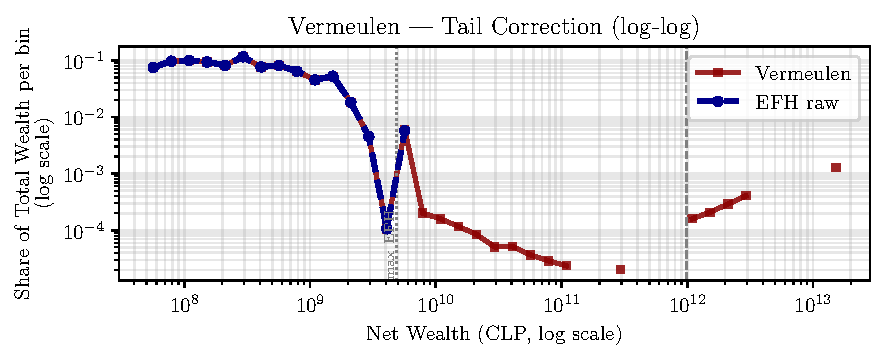
\includegraphics[width=0.95\textwidth]{../../figures/p2/vermeulen_tail.pdf}
    \caption{Tail density (log-log): share per bin, EFH raw vs.\ Vermeulen.}\label{fig:ver_tail}
\end{figure}


\paragraph{Final Comparison.} Table~\ref{tab:shares-corr} compares raw and corrected shares. Both Figure~\ref{fig:ver_tail} and Figure~\ref{fig:wealth-comparison} use $\hat{\alpha}_{\text{MLE}}=1.86$ at $w_{\min}=380$m ($\lambda^{F}\approx 0.48$).
\begin{table}[H]
    \centering
    \caption{Wealth shares: raw vs.\ Vermeulen (380m, MLE $\hat{\alpha}=1.86$)}\label{tab:shares-corr}
    \begin{tabular}{lccc}
        \toprule
        & bottom50 & top10 & top1 \\
        \midrule
        Raw & 6.8\% & 51.4\% & 14.6\% \\
        Corrected & 5.6\% & 53.6\% & 15.8\% \\
        \bottomrule
    \end{tabular}
\end{table}
Correction shifts about 1pp to the top.

\begin{figure}[H]
    \centering
    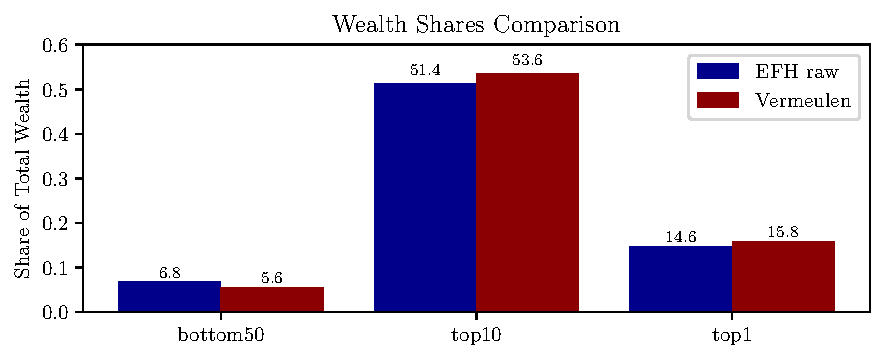
\includegraphics[width=0.95\textwidth]{../../figures/p2/shares_vermeulen.pdf}
    \caption{Wealth shares raw vs.\ Vermeulen-corrected (380m, MLE $\hat{\alpha}=1.86$): bottom50, top10, top1.}\label{fig:wealth-comparison}
\end{figure}

The effect is modest compared to Vermeulen (2018) (e.g.\ Italy +6pp) because $\hat{\alpha}=1.86$ implies a fatter tail than Reg, yet still thin: the Pareto mean $\hat{\alpha}/(\hat{\alpha}-1)\times w_{\min}$ adds little mass beyond 4.9b. Had we used $\hat{\alpha}_{\text{Reg}}=2.15$ at p99, the top 1\% gain would be roughly half, as suggested by the steeper slope in Figure~\ref{fig:pareto_qq}. The counterpart is the bottom 50\% falling from 6.8\% to 5.6\%: fixing the denominator with $W^{\text{NA}}$ while adding top wealth mechanically dilutes the bottom. In short, the survey captures the middle well but misses the extreme right, and the correction size hinges entirely on $\hat{\alpha}$.